Es muy probable que al menos un factor de un número sea $B$-powersmooth para $B$ pequeños. $B$-powersmooth significa que cada potencia primaria $d^k$ que divide $p-1$ es es como máximo $B$. Por ejemplo, la factorización prima de $4817191$ es $1303 \cdot 3697$ . Y los factores son $31$-powersmooth y $16$-powersmooth respetablemente, porque  $1303 - 1 = 2 \cdot 3 \cdot 7 \cdot 31$ y $3697 - 1 = 2^4 \cdot 3 \cdot 7 \cdot 11$. En 1974, John Pollard inventó un método para extraer $B$-powersmooth factores  de un número compuesto.

La idea surge del pequeño teorema de Fermat . Sea una factorización de $n$  ser $n = p \cdot q$ . Dice que si $a$ es coprimo a $p$ , se cumple la siguiente afirmación:

$$a^{p - 1} \equiv 1 \pmod{p}$$

Esto también significa que

$$a^{(p - 1)^k} \equiv a^{k \cdot (p - 1)} \equiv 1 \pmod{p}.$$

Entonces para cualquier $M$ con $p - 1 ~|~ M$ sabemos que $a^M \equiv 1$. Esto significa que  $a^M - 1 = p \cdot r$, y por eso también $p ~|~ \gcd(a^M - 1, n)$.

Por lo tanto, si $p-1$ por un factor $p$ de $n$ divide $M$, podemos extraer un factor usando el algoritmo de Euclides.

Está claro que el más pequeño $M$ que es múltiplo de cada $B$-powersmooth numero es $\text{lcm}(1,~2~,3~,4~,~\dots,~B)$. O alternativamente:

 $$M = \prod_{\text{prime } q \le B} q^{\lfloor \log_q B \rfloor}$$
 
Aviso, si $p-1$ divide $M$ para todos los factores primos $p$ de $n$ , entonces $\gcd(a^M - 1, n)$ solo será $n$. En este caso no recibimos ningún factor. Por lo tanto, intentaremos realizar el $\gcd$ varias veces, mientras calculamos $M$.

Algunos números compuestos no tienen $B$-powersmooth factores para pequeños B . Por ejemplo, los factores del número compuesto $100~000~000~000~000~493 = 763~013 \cdot 131~059~365~961$ son $190~753$-powersmooth y $1~092~161~383$-powersmooth. Tendremos que elegir $B >= 190~753$ para factorizar el número

Observe que este es un algoritmo probabilístico. Una consecuencia de esto es que existe la posibilidad de que el algoritmo no pueda encontrar
ningún factor.

\subsubsection{Algoritmo $\rho$ de Pollard}

El algoritmo Rho de Pollard es otro algoritmo de factorización de John Pollard.  Sea la factorización prima de un número $n = p q$. El algoritmo analiza una secuencia pseudoaleatoria. $\{x_i\} = \{x_0,~f(x_0),~f(f(x_0)),~\dots\}$ dónde $f$ es una función polinómica, generalmente $f(x) = (x^2 + c) \bmod n$  es elegido con $c = 1$.

En este caso no nos interesa la secuencia $\{x_i\}$ . Estamos más interesados en la secuencia. $\{x_i \bmod p\}$. Desde $f$ es una función polinómica y todos los valores están en el rango $[0;~p)$, esta secuencia eventualmente convergerá en un bucle. La paradoja del cumpleaños en realidad sugiere que el número esperado de elementos es $O(\sqrt{p})$ hasta que comience la repetición. Si $p$ es más pequeña que $\sqrt{n}$, la repetición probablemente comenzará en $O(\sqrt[4]{n})$.


Aquí hay una visualización de tal secuencia $\{x_i \bmod p\}$ con $n = 2206637$, $p = 317$, $x_0 = 2$ y $f(x) = x^2 + 1$. Por la forma de la secuencia se puedever muy claramente por qué el algoritmo se llama algoritmo $\rho$ de Pollard.

% TODO: \usepackage{graphicx} required
\begin{figure}[h!]
	\centering
	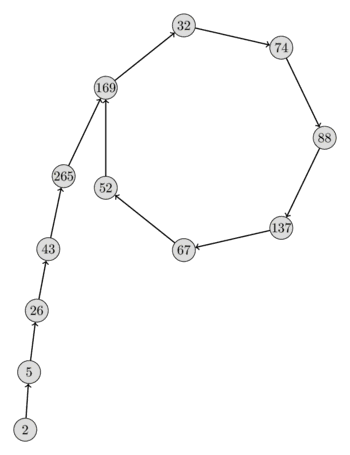
\includegraphics[width=0.35\linewidth]{img/pollard_rho}
	
	\label{fig:pollardrho}
\end{figure}


Sin embargo, todavía queda una pregunta abierta. ¿Cómo podemos explotar las propiedades de la secuencia? $\{x_i \bmod p\}$ a nuestra ventaja sin siquiera saber el número $p$ ¿sí mismo?

En realidad es bastante fácil. Hay un ciclo en la secuencia $\{x_i \bmod p\}_{i \le j}$ si y sólo si hay dos índices $s, t \le j$ tal que $x_s \equiv x_t \bmod p$. Esta ecuación se
puede reescribir como $x_s - x_t \equiv 0 \bmod p$ que es lo mismo que $p ~|~ \gcd(x_s - x_t, n)$.

Por tanto, si encontramos dos índices $s$  y $t$ con $g = \gcd(x_s - x_t, n) > 1$ , hemos encontrado un ciclo y también un factor  $g$ de $n$. Es posible que $g = n$.
En este caso no hemos encontrado un factor adecuado, por lo que debemos repetir el algoritmo con un parámetro diferente (valor inicial diferente $x_0$ , constante diferente $c$ en la función polinómica $f$ ).

Para encontrar el ciclo, podemos utilizar cualquier algoritmo de detección de ciclo común.

\subsubsection{Algoritmo de búsqueda de ciclos de Floyd}
Este algoritmo encuentra un ciclo utilizando dos punteros que se mueven sobre la secuencia a 
diferentes velocidades. Durante cada iteración, el primer puntero avanzará un elemento, mientras 
que el segundo puntero avanzará a todos los demás elementos. Usando esta idea es fácil observar que 
si hay un ciclo, en algún momento el segundo puntero se encontrará con el primero durante los 
bucles. Si la duración del ciclo es $\lambda$ y el $\mu$ es el primer índice en el que comienza el 
ciclo, entonces el algoritmo se ejecutará en O$(\lambda + \mu)$ tiempo.

Este algoritmo también se conoce como algoritmo de la liebre y la tortuga , basado en el cuento en el que una tortuga (el puntero lento) y una liebre (el puntero más rápido) tienen una carrera.

De hecho, es posible determinar el parámetro $\lambda$ y $\mu$ usando este algoritmo (también en 
O($\lambda + \mu$) tiempo y O$(1)$ espacio). Cuando se detecta un ciclo, el algoritmo devolverá 
verdadero . Si la secuencia no tiene un ciclo, entonces la función se repetirá sin cesar. Sin 
embargo, esto se puede evitar utilizando el algoritmo Rho de Pollard.

La siguiente tabla muestra los valores de $x$ y $y$ durante el algoritmo para $n = 2206637$ , $x_0 = 2$ y $c = 1$.

$$
\newcommand\T{\Rule{0pt}{1em}{.3em}}
\begin{array}{|l|l|l|l|l|l|}
	\hline
	i & x_i \bmod n & x_{2i} \bmod n & x_i \bmod 317 & x_{2i} \bmod 317 & \gcd(x_i - x_{2i}, n) \\
	\hline
	0   & 2       & 2       & 2       & 2       & -   \\
	1   & 5       & 26      & 5       & 26      & 1   \\
	2   & 26      & 458330  & 26      & 265     & 1   \\
	3   & 677     & 1671573 & 43      & 32      & 1   \\
	4   & 458330  & 641379  & 265     & 88      & 1   \\
	5   & 1166412 & 351937  & 169     & 67      & 1   \\
	6   & 1671573 & 1264682 & 32      & 169     & 1   \\
	7   & 2193080 & 2088470 & 74      & 74      & 317 \\
	\hline
\end{array}
$$

Como se dijo anteriormente, si $n$ es compuesto y el algoritmo devuelve $n$ como factor, hay que repetir el procedimiento con diferentes parámetros $x_0$ y $c$. Por ejemplo, la elección $x_0 = c = 1$ no factorizará $25 = 5 \cdot 5$. El algoritmo volverá $25$. Sin embargo, la elección $x_0 = 1$, $c = 2$ lo factorizará.


\subsubsection{Algoritmo de Brent}

Brent implementa un método similar al de Floyd, utilizando dos punteros. La diferencia es que en lugar de avanzar los punteros uno y dos lugares respectivamente, avanzan potencias de dos. Tan pronto como $2^i$ es mayor que $\lambda$ y $\mu$ , encontraremos el ciclo.